
\documentclass[acmlarge,nonacm=true]{acmart}
\usepackage{adjustbox}
\usepackage{multirow}
\usepackage{graphicx}
\usepackage{afterpage}
\usepackage{subcaption}

\newcommand\blankpage{%
	\null
	\thispagestyle{empty}%
	\addtocounter{page}{-1}%
	\newpage}

%%
%% \BibTeX command to typeset BibTeX logo in the docs
\AtBeginDocument{%
  \providecommand\BibTeX{{%
    \normalfont B\kern-0.5em{\scshape i\kern-0.25em b}\kern-0.8em\TeX}}}


\begin{document}
	
	\begin{titlepage}
		\begin{center}
			\vspace*{1cm}
			
\includegraphics[width=0.7\textwidth]{fig/ntu_logo}
			\vspace{0.8cm}
			\linebreak
			\Huge
			\textbf{Experiment 3: Parametric Solids}
			
			\vspace{0.5cm}
			\LARGE
			CZ2003 Computer Graphics and Visualization
			
			\vspace{1.5cm}
			\textbf{SS3}\\
			
			\begin{table}[h]
				\begin{tabular}{lc}
					Name & Matric Number \\\hline
					Pang Yu Shao & U17216\underline{\textbf{80}}D \\
				\end{tabular}
			\end{table}
			
			
			
			\vfill
			
			\vspace{0.8cm}
			
			
			
			\Large
			SCHOOL OF COMPUTER SCIENCE AND ENGINEERING\\
			NANYANG TECHNOLOGICAL UNIVERSITY\\
			SINGAPORE\\
			9th March 2021
			
		\end{center}
	\end{titlepage}

 

%%
%% The "title" command has an optional parameter,
%% allowing the author to define a "short title" to be used in page headers.
\title{CZ2003 Computer Graphics and Visualization}

%%
%% The "author" command and its associated commands are used to define
%% the authors and their affiliations.
%% Of note is the shared affiliation of the first two authors, and the
%% "authornote" and "authornotemark" commands
%% used to denote shared contribution to the research.


\author{Pang Yu Shao}
\email{C170134@e.ntu.edu.sg}
\affiliation{\institution{Nanyang Technological University}}

%%
%% By default, the full list of authors will be used in the page
%% headers. Often, this list is too long, and will overlap
%% other information printed in the page headers. This command allows
%% the author to define a more concise list
%% of authors' names for this purpose.
\renewcommand{\shortauthors}{Pang Yu Shao}






%%
%% This command processes the author and affiliation and title
%% information and builds the first part of the formatted document.

% \begin{teaserfigure}
% 	\includegraphics[width=\textwidth]{bccell}
% 	\caption{Breast Cancer Cell. Photograph by National Cancer Institute [Public domain], via Wikimedia
% 		Commons. (\url{https://w.wiki/kS3}).}
% 	\Description{A breast cancer cell seen through an electron microscope.}
% \end{teaserfigure}
% \maketitle



\tableofcontents
\newpage
\section{Defining Solids Parametrically}
\subsection{Solid Box with Sides Parallel to Coordinate Planes and Two Defined Vertices}
The solid box is defined with two opposite vertices: \((N,\ 0,\ M)\) and \((N+M,\  M,\  2(N+M))\)\\ 
Since \(N = 8\) and \(M = 10\),
The two vertices are: \((8,\ 0,\ 10)\) and \((18,\  10,\  36)\)\\\\
Therefore, the following parametric functions defining the solid box can be obtained:\\
\(x(u,v,w) = \mathbf{8 + 10u}\)\\
\(y(u,v,w) = \mathbf{10v}\)\\
\(z(u,v,w) = \mathbf{10 + 26w}\)\\
\(\mathbf{u,v,w \in [0,1]}\)

\begin{figure}[H]
	\begin{subfigure}{.33\textwidth}
	  \centering
	  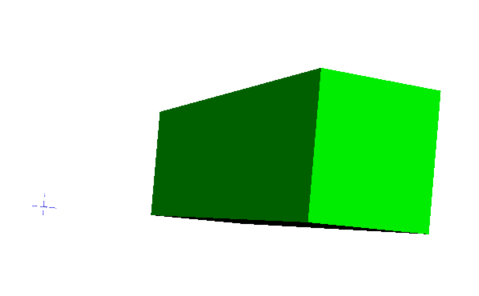
\includegraphics[width=.8\linewidth]{fig/1a1_1_1}
	  \caption{Resolution: 1 1}
	\end{subfigure}%
	\begin{subfigure}{.33\textwidth}
	  \centering
	  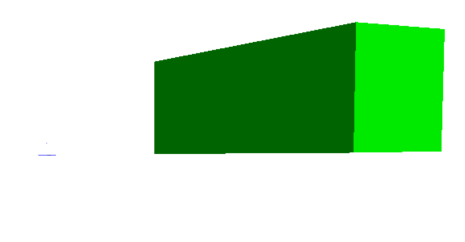
\includegraphics[width=.8\linewidth]{fig/1a10_10_10}
	  \caption{Resolution: 10 10}
	\end{subfigure}
	\begin{subfigure}{.33\textwidth}
		\centering
		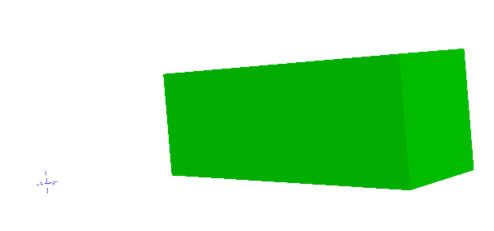
\includegraphics[width=.8\linewidth]{fig/1a100_100_100}
		\caption{Resolution: 1000 1000}
	  \end{subfigure}
	\caption{Plots of the Solid Box defined in "\textbf{1a.wrl}" with differing resolutions}
	\label{fig:1a}
\end{figure}
As seen in Fig. \ref{fig:1a} above, a sampling resolution of \textbf{1} for u,v and w is 
sufficient for visualizing the solid as it has no curvature and having a higher resolution would
produce the exact same visualization.

\subsection{Solid Three-Sided Pyramid}
To define the three-sided pyramid, we first define the triangular base, then scale the base up to the apex with
an additional degree of freedom. First, we use the formula for defining Bilinear Surface Parametrically to 
define the triangular base, and we set two of the points to be the same point, essentially resulting in a 
Triangular polygon.\\\\
\(P = P1 + u(P2-P1) + v(P3-P1+u(P4-P3-(P2-P1)))\)\\
Let P4 = P3, we get:\\
\(P = P1 + u(P2 - P1) + v(P3 - P1) + uv(P1 - P2)\)\\
Therefore, with the 3 points \((0, 0, 0),\ (N, 0, 0),\ (0, 0, M)\), we get:\\
\(x(u,v) = uN - uvN = \mathbf{8u - 8uv}\)\\
\(y(u,v) = 0\)\\
\(z(u,v) = vM = \mathbf{10v}\)\\
\(\mathbf{u,v \in [0,1]}\)\\\\

Next, we scale the functions for \(x\) and \(z\) with the third degree of freedom, \(w\). We get:\\
\(x(u,v,w) = \mathbf{(8u - 8uv) - (8u - 8uv)w}\)\\
\(y(u,v,w) = (N+M)w = \textbf{18w}\)\\
\(z(u,v,w) = \mathbf{10v - 10vw}\)\\
\(\mathbf{u,v,w \in [0,1]}\)\\\\
\begin{figure}[H]
	\begin{subfigure}{.33\textwidth}
	  \centering
	  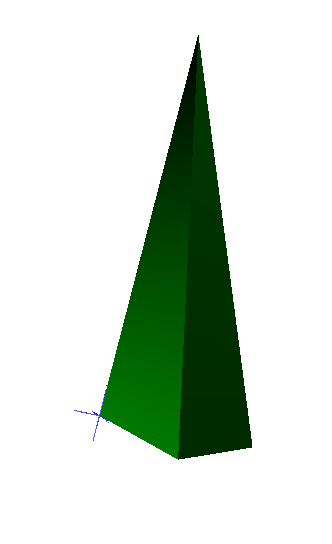
\includegraphics[width=.8\linewidth]{fig/1b1_1_1}
	  \caption{Resolution: 1 1 1}
	\end{subfigure}%
	\begin{subfigure}{.33\textwidth}
	  \centering
	  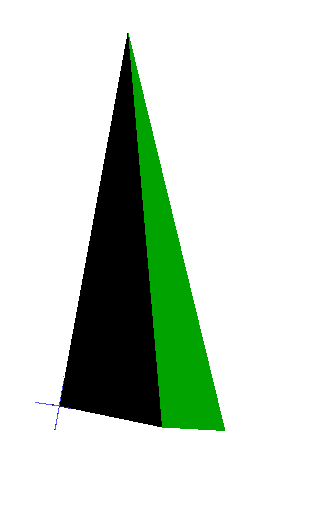
\includegraphics[width=.8\linewidth]{fig/1b10_10_10}
	  \caption{Resolution: 10 10 10}
	\end{subfigure}
	\begin{subfigure}{.33\textwidth}
		\centering
		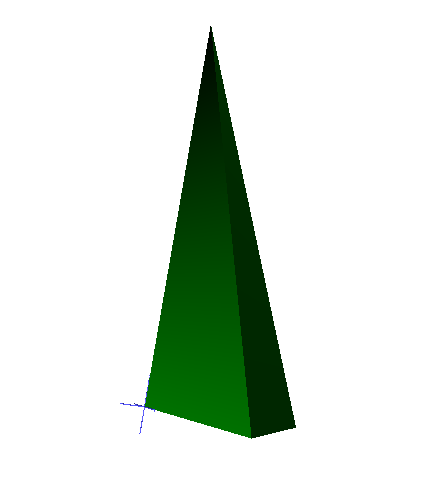
\includegraphics[width=.8\linewidth]{fig/1b100_100_100}
		\caption{Resolution: 100 100 100}
	  \end{subfigure}
	\caption{Plots of the Three-Sided Pyramid defined in "\textbf{1b.wrl}" with differing resolutions}
	\label{fig:1b}
\end{figure}

As seen in Fig. \ref{fig:1b} above, a sampling resolution of \textbf{1} for both u and v is 
sufficient for drawing the triangular polygon as it has no curvature and having a higher resolution would
produce the exact same drawing.


\subsection{Half of Origin-Centered Solid Sphere}
\label{section:1c}
To define the half-sphere with a radius \textbf{8}, we first define a 2D semi-circle surface with the following parametric functions:\\
\(x(u,v) = 8v*cos(-\pi + \pi u)\)\\
\(y(u,v) = 8v*sin(-\pi + \pi u)\)\\
\(z(u,v) = 0\)\\
\(u,v \in [0,1]\)

Thus, the half-sphere can be obtained by rotating the semi-circle about the z-axis with the another degree of freedom.
The following functions can be obtained:\\
\(x(u,v,w) = (8v*cos(-\pi + \pi u))*sin(\pi w)\)\\
\(y(u,v,w) = 8v*sin(-\pi + \pi u)\)\\
\(z(u,v,w) = (8v*cos(-\pi + \pi u))*cos(\pi w)\)\\
\(u,v,w \in [0,1]\)

\begin{figure}[H]
	\begin{subfigure}{.33\textwidth}
	  \centering
	  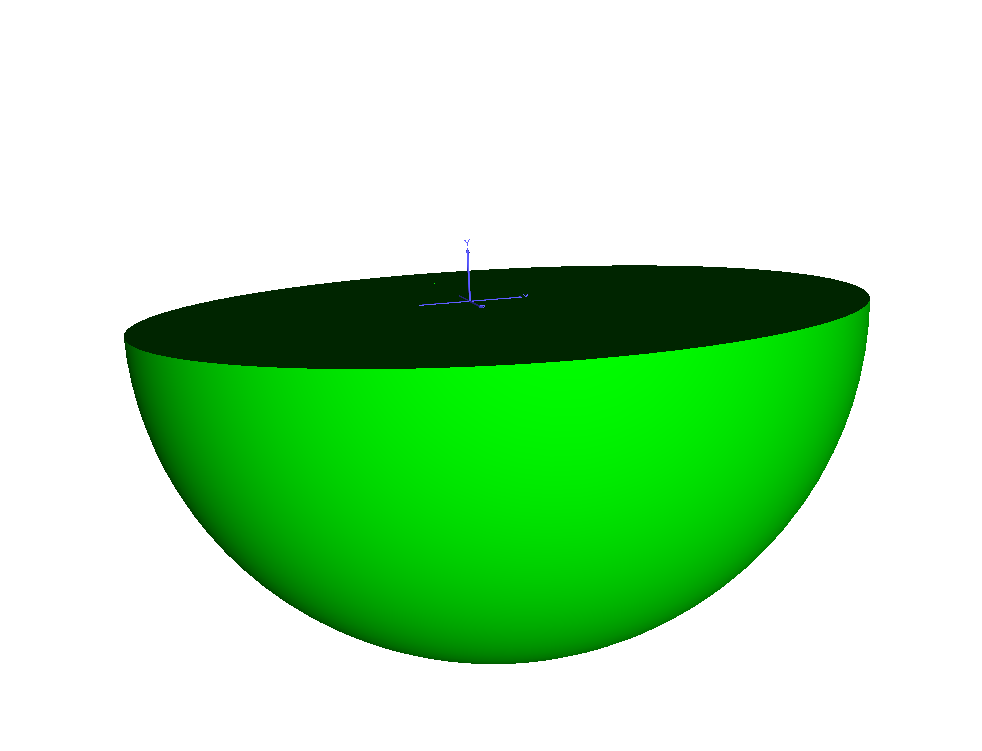
\includegraphics[width=.8\linewidth]{fig/1c50_50_50}
	  \caption{Resolution: 50 50 50}
	\end{subfigure}%
	\begin{subfigure}{.33\textwidth}
	  \centering
	  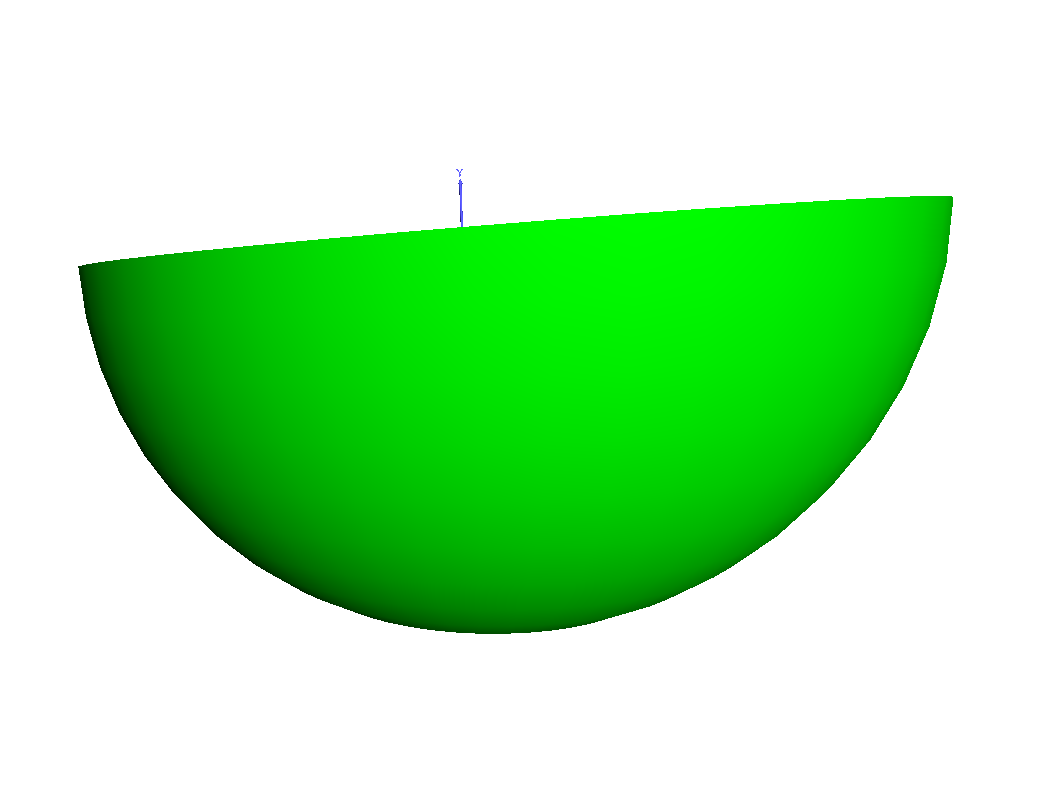
\includegraphics[width=.8\linewidth]{fig/1c25_25_25}
	  \caption{Resolution: 25 25 25}
	\end{subfigure}
	\begin{subfigure}{.33\textwidth}
		\centering
		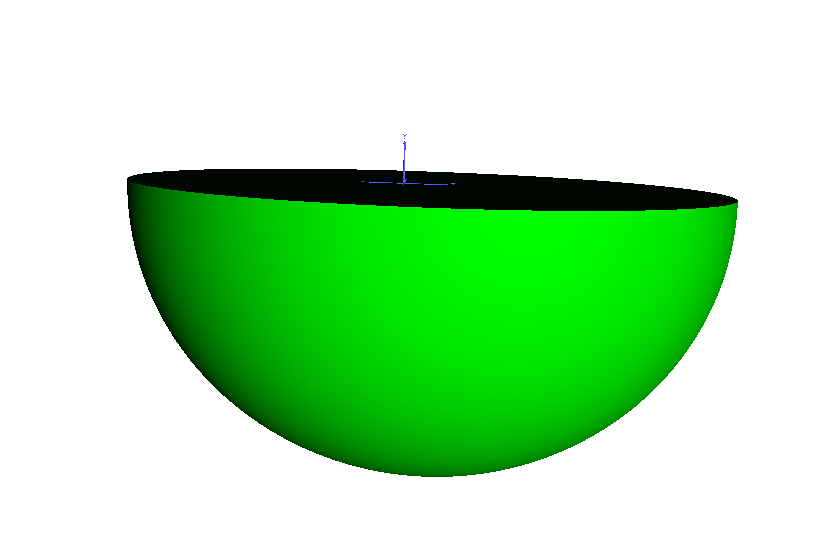
\includegraphics[width=.8\linewidth]{fig/1c100_100_100}
		\caption{Resolution: 100 100 100}
	  \end{subfigure}
	\caption{Plots of the Half-Sphere defined in "\textbf{1c.wrl}" with differing resolutions}
	\label{fig:1c}
\end{figure}

As seen in Fig. \ref{fig:1c} above, the best resolution obtained was \textbf{50} for u, v and w.
By decreasing the resolution to 25, the interpolations could be seen on the curvature when zoomed in. 
When the resolution was increased instead to 100, no visible difference could be seen between that and when the resolution was 50.

\subsection{Half of Origin-Centered Torus}
\label{section:1d}
Similar to the solid defined in \ref{section:1c}, A 2D semi-circle of radius \textbf{8/5} 
is defined first, next an offset of \textbf{8} is applied to the x function. Lastly, the torus is formed by
rotational sweeping about y-axis. Therefore, the following functions can be obtained:\\
\(x(u,v,w) = \mathbf{(8 + 1.6v*cos(\pi u))*sin(2\pi w)}\)\\
\(y(u,v,w) = \mathbf{1.6v*sin(\pi u)}\)\\
\(z(u,v,w) = \mathbf{(8 + 1.6v*cos(\pi u))*cos(2\pi w)}\)\\
\(u,v,w \in [0,1]\)
\begin{figure}[H]
	\begin{subfigure}{.33\textwidth}
	  \centering
	  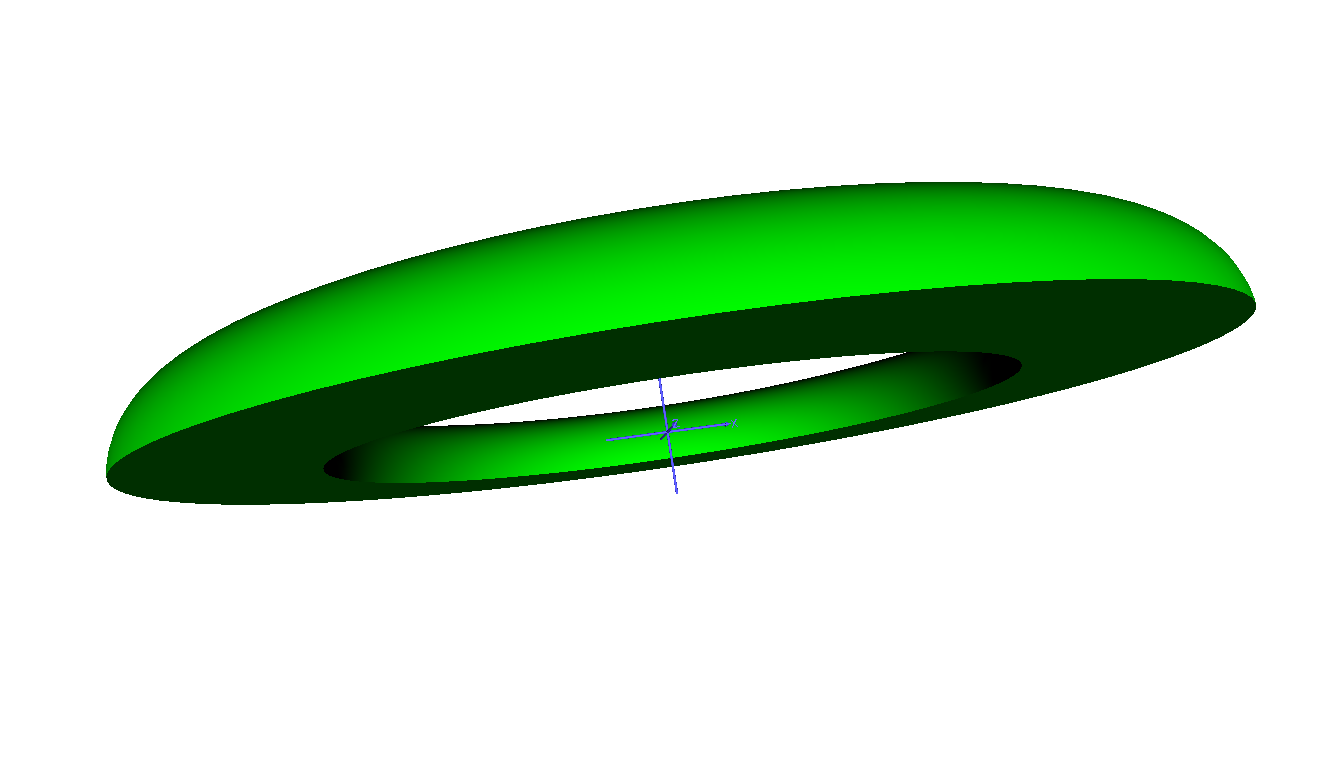
\includegraphics[width=.8\linewidth]{fig/1d100_100_100.PNG}
	  \caption{Resolution: 100 100 100}
	\end{subfigure}%
	\begin{subfigure}{.33\textwidth}
	  \centering
	  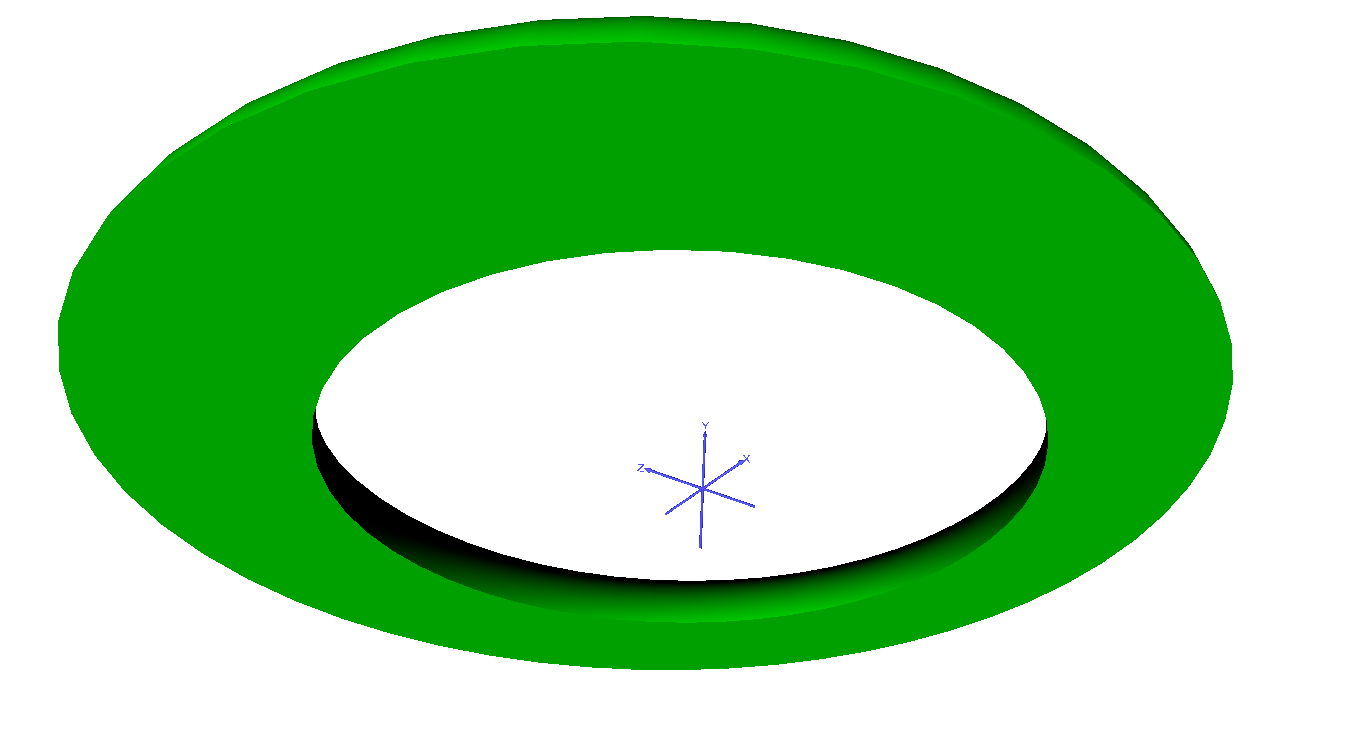
\includegraphics[width=.8\linewidth]{fig/1d50_50_50.PNG}
	  \caption{Resolution: 50 50 50}
	\end{subfigure}
	\begin{subfigure}{.33\textwidth}
		\centering
		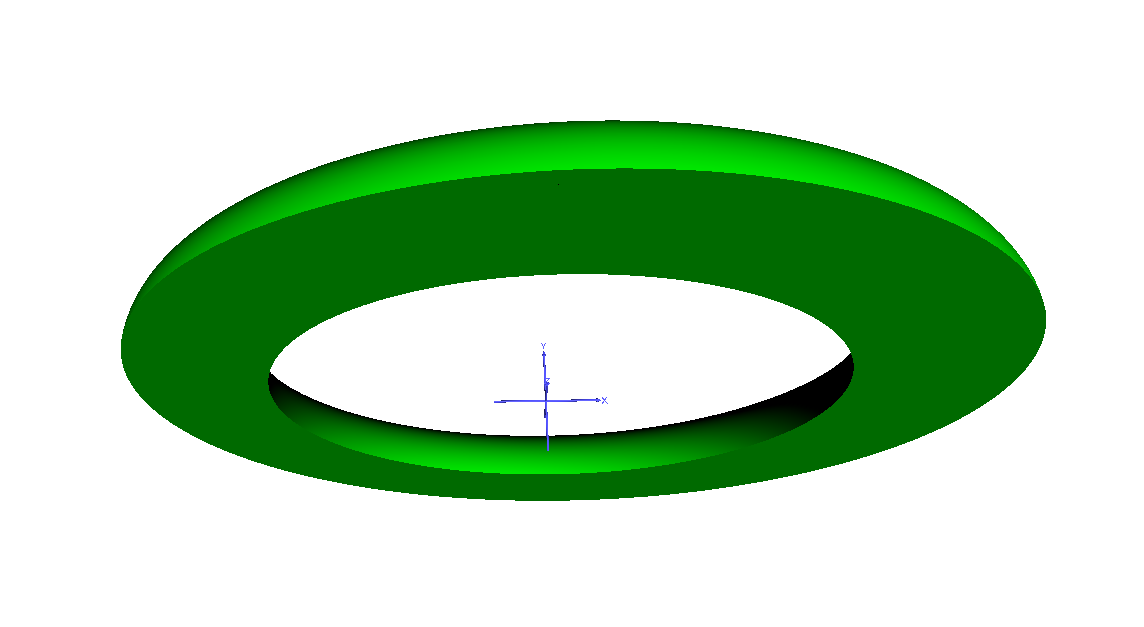
\includegraphics[width=.8\linewidth]{fig/1d200_200_200.PNG}
		\caption{Resolution: 200 200 200}
	  \end{subfigure}
	\caption{Plots of the Half-Torus defined in "\textbf{1d.wrl}" with differing resolutions}
	\label{fig:1d}
\end{figure}

As seen in Fig. \ref{fig:1d} above, the best resolution obtained was \textbf{100} for u,v and w.
By decreasing the resolution to 50, the interpolations could be seen on the curvature when zoomed in. When the resolution was 
increased instead to 200, no visible difference could be seen between that and when the resolution was 100.

\pagebreak
\section{Defining Solid by Translational Sweeping of Surface}
We obtain the equations of the curve from lab 2:

\begin{displaymath}
	\mathbf{x(u,v) = -10.4 + 26.4u}
\end{displaymath}
\begin{displaymath}
	\mathbf{y(u,v) = tanh(-10.4 + 26.4u)}
\end{displaymath}
\begin{displaymath}
	\mathbf{z(u,v) = -8 + 18v}
\end{displaymath}
\begin{displaymath}
	u,v \in [0,1]
\end{displaymath}
To obtain a solid by translational sweeping of the surface, we can introduce the w parameter in the function of Y.
Therefore, we get:\\
\begin{displaymath}
	\mathbf{x(u,v,w) = -10.4 + 26.4u}
\end{displaymath}
\begin{displaymath}
	\mathbf{y(u,v,w) = (-7 + 26w)+tanh(-10.4 + 26.4u)}
\end{displaymath}
\begin{displaymath}
	\mathbf{z(u,v,w) = -8 + 18v}
\end{displaymath}
\begin{displaymath}
	u,v,w \in [0,1]
\end{displaymath}

\begin{figure}[H]
	\begin{subfigure}{.33\textwidth}
	  \centering
	  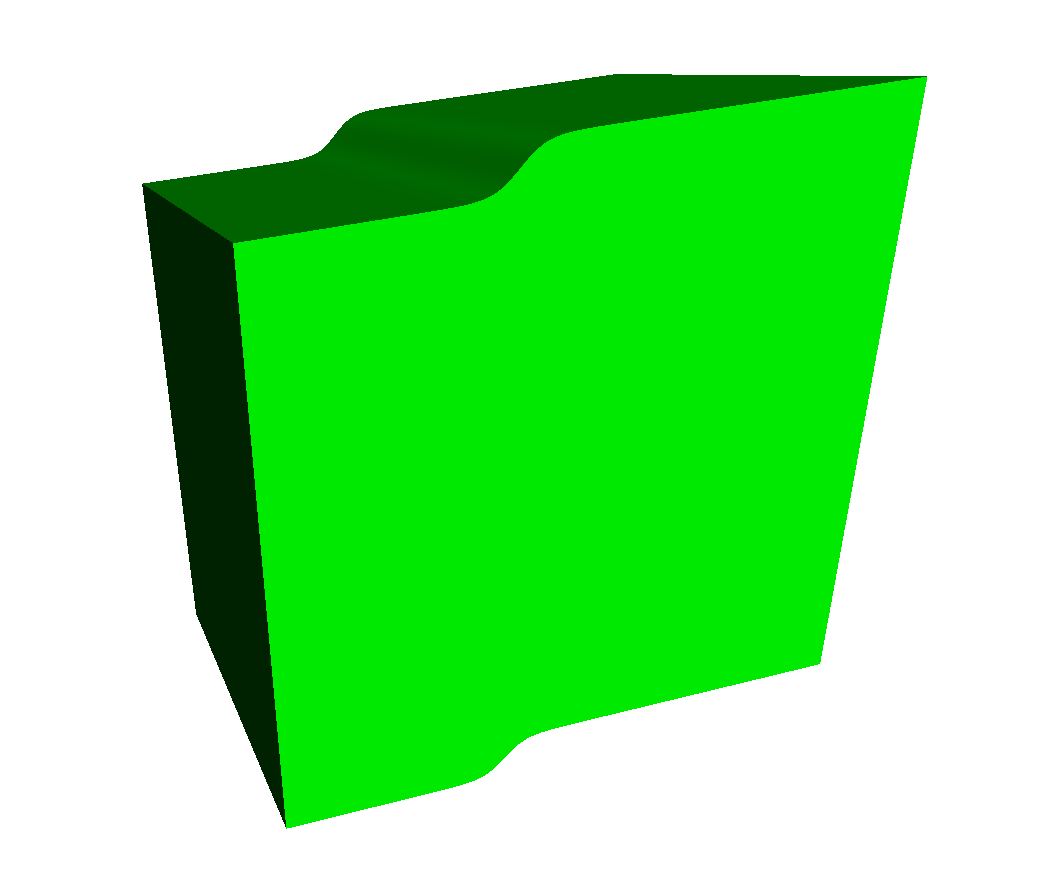
\includegraphics[width=.8\linewidth]{fig/2_200_1_1}
	  \caption{Resolution: 200 1 1}
	\end{subfigure}%
	\begin{subfigure}{.33\textwidth}
	  \centering
	  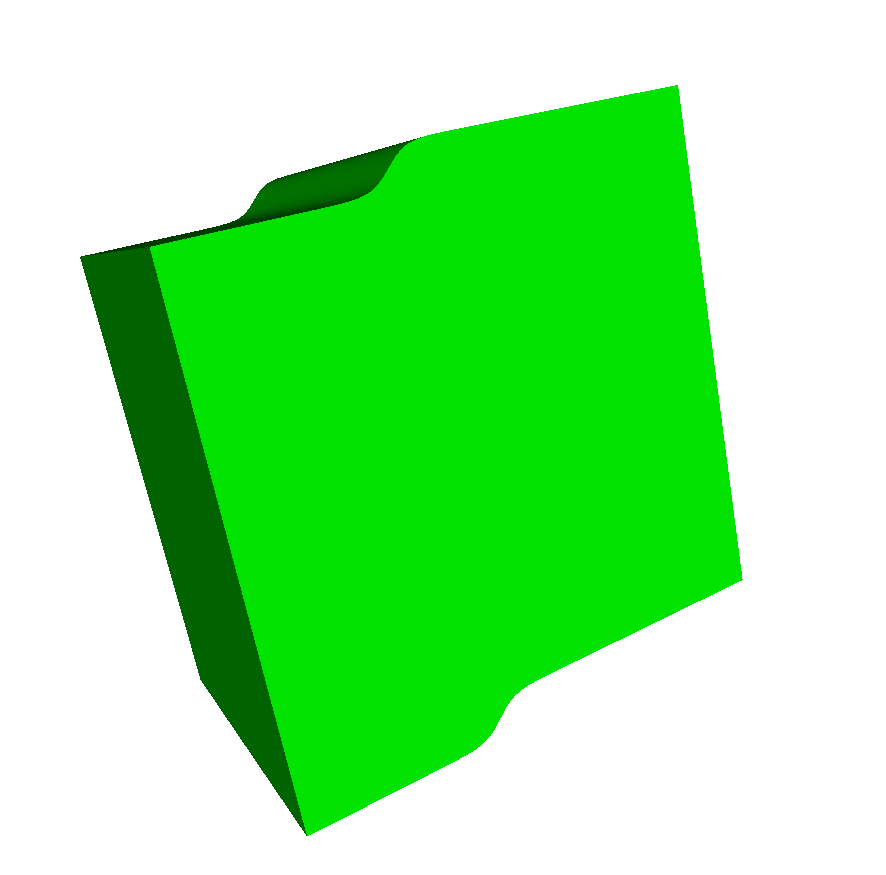
\includegraphics[width=.8\linewidth]{fig/2_100_1_1}
	  \caption{Resolution: 100 1 1}
	\end{subfigure}
	\begin{subfigure}{.33\textwidth}
		\centering
		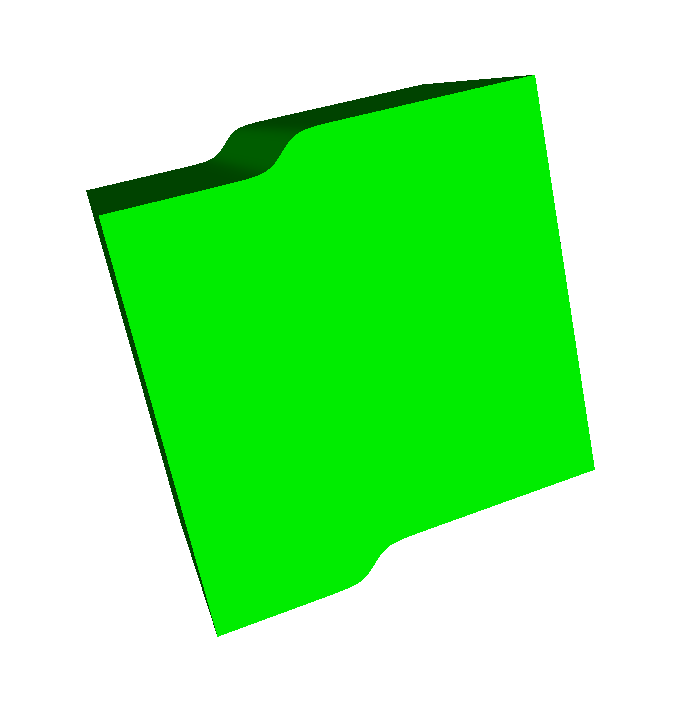
\includegraphics[width=.8\linewidth]{fig/2_1000_1_1}
		\caption{Resolution: 1000 1 1}
	  \end{subfigure}
	\caption{Plots of the Solid defined in "\textbf{2.wrl}" with differing resolutions}
	\label{fig:2}
\end{figure}

The sampling resolution for v and w is chosen to be 1 as the parameters are responsible for the straight line sweep.
As seen in Fig. \ref{fig:2} above, the best resolution obtained was \textbf{200, 1, 1} for u, v and w respectively.
By decreasing the resolution to 100 for u, the interpolations could be seen on the curvature when zoomed in. When the resolution of u was 
increased instead to 1000, no visible difference could be seen between that and when the resolution was 200.
\pagebreak
\section{Defining Solid by Linear Sweeping of Polar Function}
We obtain the equations of the Surface in lab 2:

\begin{displaymath}
	\mathbf{x(u,v) =  ((8 - 15cos(2\pi u))cos(2\pi u)-8)sin(\frac{3\pi}{20} - \frac{\pi}{8}v)}
\end{displaymath}\\
\begin{displaymath}
	\mathbf{y(u,v) =  (8 - 15cos(2\pi u))sin(2\pi u)}
\end{displaymath}\\
\begin{displaymath}
	\mathbf{z(u,v) =  ((8 - 15cos(2\pi u))cos(2\pi u)-8)cos(\frac{3\pi}{20} - \frac{\pi}{8}v)}
\end{displaymath}
\begin{displaymath}
	u,v \in [0, 1]
\end{displaymath}

In order to fill in the solid, recall that the surface is defined with a polar function. Therefore, to fill it in, 
sweeping is done on the polar function: \(r = (8 - 15cos(2\pi u))\) by multiplying it with the third degree of freedom, w.\\
Therefore, the following equations are obtained for the solid:\\
\begin{displaymath}
	\mathbf{x(u,v,w) =  (((8 - 15cos(2\pi u))*w)cos(2\pi u)-8)sin(\frac{3\pi}{20} - \frac{\pi}{8}v)}
\end{displaymath}\\
\begin{displaymath}
	\mathbf{y(u,v,w) =  ((8 - 15cos(2\pi u))*w)sin(2\pi u)}
\end{displaymath}\\
\begin{displaymath}
	\mathbf{z(u,v,w) =  (((8 - 15cos(2\pi u))*w)cos(2\pi u)-8)cos(\frac{3\pi}{20} - \frac{\pi}{8}v)}
\end{displaymath}
\begin{displaymath}
	u,v,w \in [0, 1]
\end{displaymath}


\begin{figure}[H]
	\begin{subfigure}{.33\textwidth}
	  \centering
	  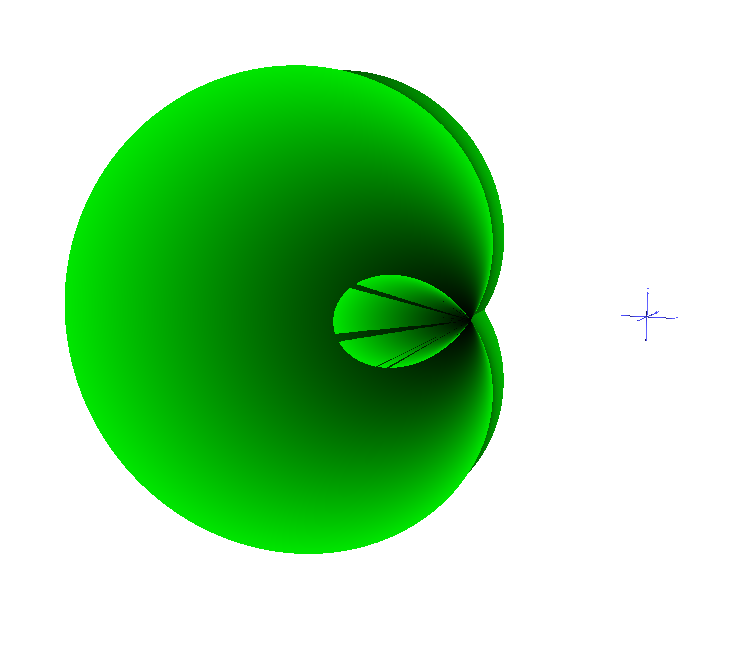
\includegraphics[width=.8\linewidth]{fig/3_200_14_1}
	  \caption{Resolution: 200 14 1}
	\end{subfigure}%
	\begin{subfigure}{.33\textwidth}
	  \centering
	  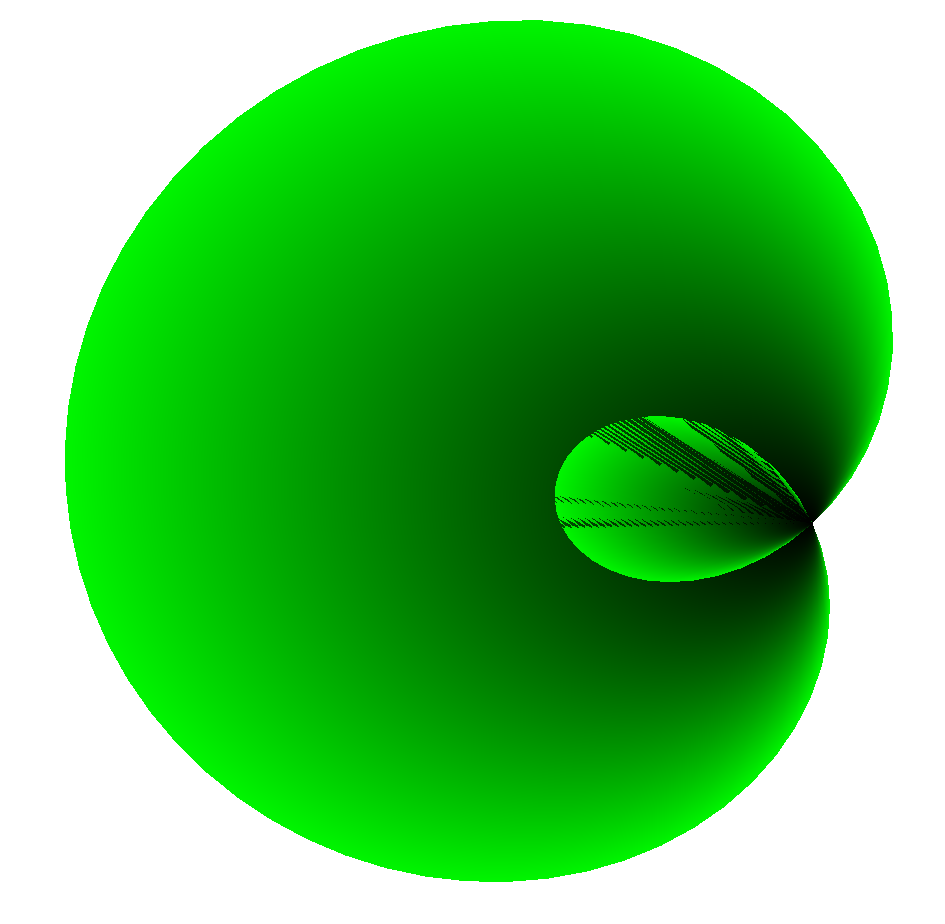
\includegraphics[width=.8\linewidth]{fig/3_100_7_1}
	  \caption{Resolution: 100 7 1}
	\end{subfigure}
	\begin{subfigure}{.33\textwidth}
		\centering
		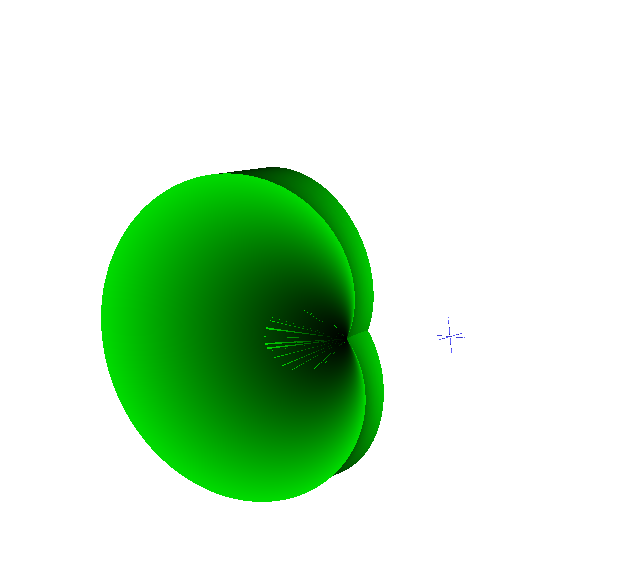
\includegraphics[width=.8\linewidth]{fig/3_400_28_1}
		\caption{Resolution: 400 28 1}
	  \end{subfigure}
	\caption{Plots of the Solid defined in "\textbf{3.wrl}" with differing resolutions}
	\label{fig:3}
\end{figure}

The sampling resolution for w is chosen to be 1 as it is just a straight line sweep. 
As seen in Fig. \ref{fig:3} above, the best resolution obtained was \textbf{200, 14, 1} for u, v and w respectively.
By decreasing the resolution to 100, 7, 1, the interpolations could be seen on the curvature when zoomed in. When the resolution was increased
instead to 400, 28, 1, no visible difference could be seen when compared to the shape defined with the resolutions 200, 14, 1.

\bibliographystyle{ACM-Reference-Format}
\newpage






\end{document}
\endinput
%%
%% End of file `sample-acmlarge.tex'.
